\documentclass{article}
\usepackage{graphicx}
\usepackage{tikz}
\usepackage{float}
\usepackage{url}
\usetikzlibrary{positioning, shapes, arrows}



\title{MS Thesis Proposal} % 
\author{Jordan Quinn}
\date{\today}


\begin{document}

\maketitle


\section{Introduction}

This thesis proposes to design an e-graph program representation and necessary extensions to equality saturation to apply to the MLton compiler. While equality saturation has shown great use as a program optimization technique, particularly in imperative languages, applying it to MLton presents challenges due to its unique Single Static Assignment (SSA) Intermediate Representation (IR) and some of the expressive features of Standard ML (SML). In particular, we must consider advanced control flow constructs, such as irreducible control flow and pattern matching, which are challenging to represent in previous e-graphs program representations without compromising equality saturation.

A related challenge is representing Algebraic Data Types (ADTs) and their use in pattern matching and decomposition. These introduce structural conditions that are difficult to model cleanly in e-graph-based frameworks. This difficulty makes it challenging to leverage equality saturation for optimization.

This project explores a hybrid approach inspired by recent work on Cranelift and Julia to address these issues. We propose a two-tier graph IR combining an e-graph, the nested tier, for expressing equivalence, and a target for equality saturation,  with a CFG skeleton, the outer tier, to track control dependencies and preserve necessary execution structure. We additionally incorporate region nodes, a construct from Lambda SSA, part of the MLIR compiler framework, to connect the e-graph with the CFG skeleton by nesting e-graph components within CFG blocks. Together, these three components aim to support equality saturation in the presence of complex control flow and rich data structures.



\section{Background}

\subsection{E-Graphs}

An E-Graph, or Equivalence Graph, is a data structure used to represent numerous equivalent terms compactly. Initially used in theorem proving~\cite{detlefs2005} and term rewriting~\cite{nelson1979}, it has since become widely used in program optimization~\cite{eqsat-lmcs}.

An E-Graph is composed of two types of components. The first is an equality node, also known as an e-node. The e-nodes are labeled nodes with child nodes. Here, the labels can indicate a value or an operation performed on the node's children, which serve as its arguments. The second component type is an equality class, also known as an e-class. An e-class is a congruence relation over nodes known to be semantically equivalent. Every node belongs to one class, but a class may contain many nodes.

\begin{figure}
    \centering
    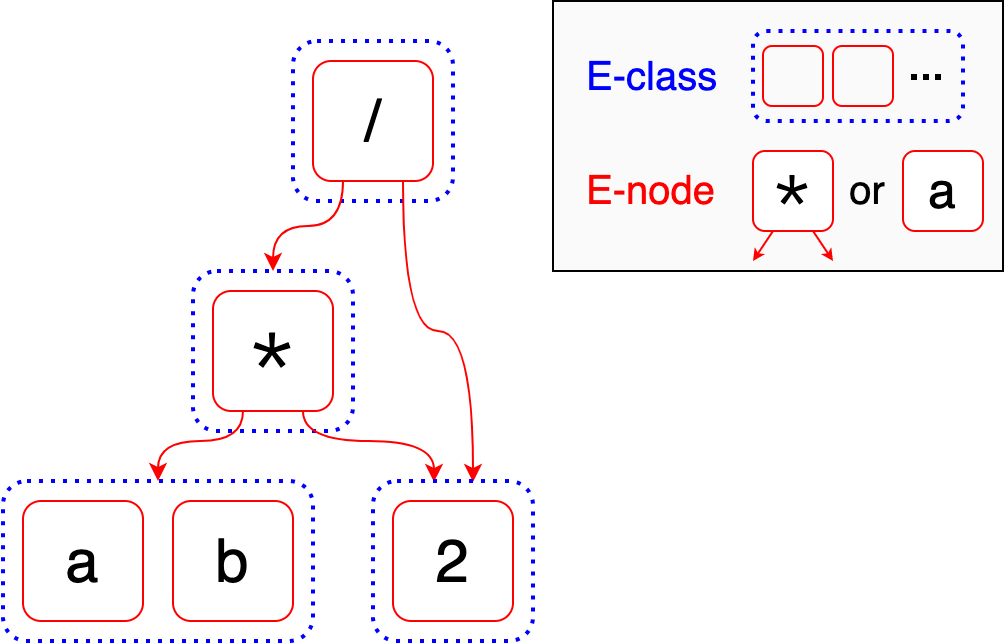
\includegraphics[width=0.5\linewidth]{assets/egraph.png}
    \caption{A simple E-Graph~\cite{k_2023}}
    \label{fig:egraph}
\end{figure}

There are a few algorithms quintessential to the e-graph data structure. The first, insertion, involves adding new terms to the e-graph. This algorithm entails creating a new equivalence class or merging it into an existing e-class, given that the inserted node is equivalent to the nodes already within the class based on the e-graph's congruence relation. The second is rebuilding. This one describes the process of restoring congruence closures after merges, which is necessary to ensure e-graph invariants hold, such as equal children implying equal parents on the same label. Third, e-matching is a pattern-matching algorithm that finds instances of a given pattern in an e-graph. These three algorithms are key in allowing for equality saturation.



\subsection{Equality Saturation}

Equality saturation~\cite{eqsat-lmcs} is an optimization technique that uses an e-graph representation to represent many equivalent programs. Instead of performing rewrites sequentially, as in traditional optimization, it builds an e-graph, which allows the exploration of multiple rewrite application orders simultaneously.

An equality saturation engine unfolds in several stages. First is the construction phase. In this phase, the initial program is translated into an e-graph-based IR. Next is the saturation phase. In this phase, we repeatedly apply rewrite rules to the e-graph. This saturation replaces the destructive rewrites in traditional optimization by adding equivalences to the graph. After there are no new rewrites, or we reach a bound, we use a heuristic to select a single, final, and hopefully better program from the e-graph. We then translate this back into the original IR.

The IRs used in the original Equality Saturation implementation are of particular note to our purpose. 


\subsubsection{E-PEGs}

A PEG (Program Expression Graph) is an IR introduced along with equality saturation~\cite{eqsat-lmcs}. The main contribution of PEG, compared to other graph-based IRs, is how it represents control flow, especially looping behavior. They borrow the gating functions from Gated SSA (GSA)~\cite{Stanier2022} but use them in a data-driven graph. See figure \ref{fig:peg} for an example PEG.

\begin{figure}
    \centering
    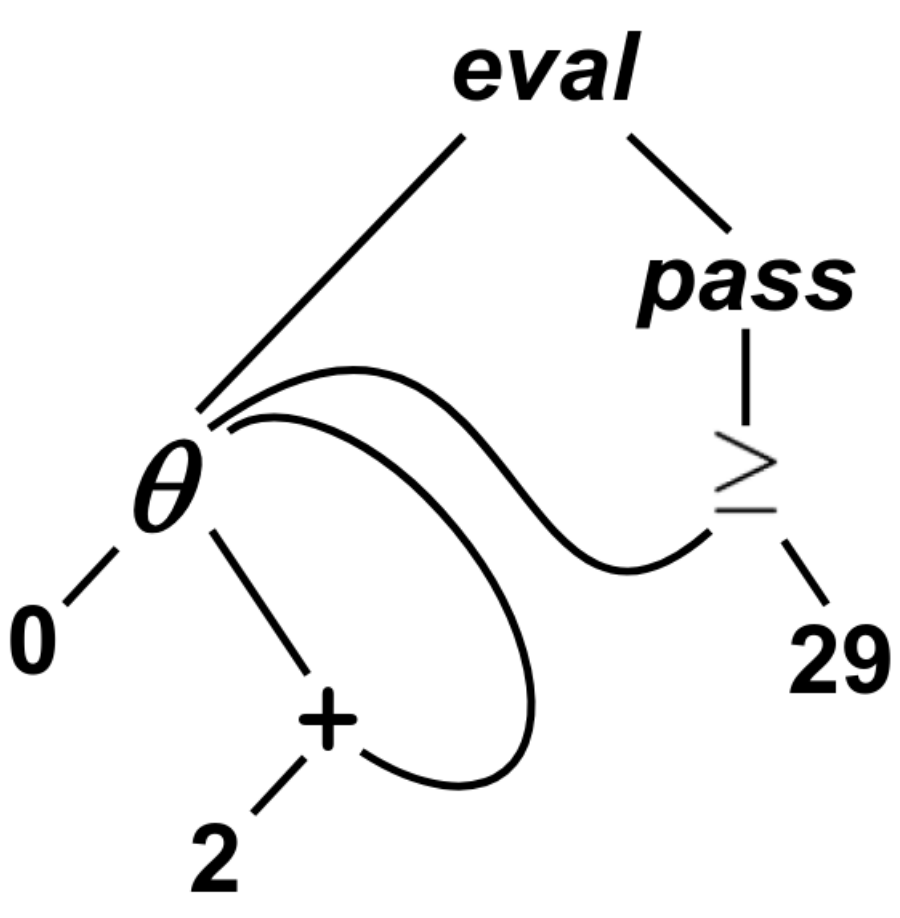
\includegraphics[width=0.25\linewidth]{assets/peg.png}
    \caption{A simple PEG~\cite{eqsat-lmcs}}
    \label{fig:peg}
\end{figure}

In particular, PEG borrows the branching and looping nodes from GSA. In PEG, the branching node $\phi$ is very similar to its GSA counterpart, serving as a simple branch on a condition with true and false branches. However, PEG is an acyclic graph that uses sequences to represent looping, whereas GSA allows back edges to represent loops. In PEGs, loop sequences are represented by complex node structures. Here, $\theta$ nodes represent loop-variant variables as lazy sequences, \verb|pass| nodes that determine the first index in a sequence that evaluates to true, and \verb|eval| nodes that select an element given a sequence and an index.

Tate et al. introduce equality classes on top of the existing PEG data structure, creating a new data structure called E-PEGs. This approach is essentially the same as in all other e-graph implementations. Here, a node's children are now e-classes, as opposed to being simply nodes as they were in PEGs, and nodes within the same class share semantic equality.

While PEGs can represent only a single version of a program, E-PEGs can represent many different equivalent representations for a program using e-classes. Then, we can select the optimal program from our E-PEG by picking within each e-class according to some heuristic.



\subsection{MLton}

MLton is a whole-program optimizing compiler for Standard ML (SML).

\subsubsection{SSA}

Single Static Assignment is an Intermediate Representation (IR) where each variable is assigned only once~\cite{Brisk2022}. It creates new variables at each necessary assignment, potentially dynamically merging variables at branch join points.

\subsubsection{MLton SSA}

In the MLton compilation process, the primary IR used for optimizations is MLton's own SSA-based IR. While this is an SSA-based IR, it differs from other SSA IRs in a few significant ways. These include, relevant to our discussion, the structure of basic blocks and the types of transfers.

First, for basic block structure, in SSA, basic blocks pass control flow along edges, potentially directed by a branch statement, and eventually merge variables at join points via $\phi$-functions. These $\phi$ functions are not actual operations during program execution but simply a mechanism used in the SSA representation. MLton SSA, however, substitutes these for basic block arguments. Here, basic blocks are labeled and take input arguments. Previous blocks can pass control flow by simply supplying another block with the proper arguments. This argument-providing strategy allows for a directly executable model.

Next, for the types of transfers, MLton allows: \verb|Call|, as in a function call; \verb|Case|, as in a case statement; \verb|Goto|, jump to another labeled basic block; \verb|Raise|, raise an exception; and \verb|Return|, an unexceptional return. While \verb|Call|, which is only a transfer when their is no result binding, \verb|Goto|, and \verb|Return| are common in SSA implementations, perhaps only now, with the new basic block arguments, we need to look at \verb|Raise| and \verb|Case|. While \verb|Raise| is not an uncommon transfer in SSA, it requires a model for exceptions and exception handling. For our case, it is helpful to think about it in terms of the \verb|Result|-style error handling of languages such as Rust that use Algebraic Data Types (ADTs) to handle exceptional computations. This directly relates to the next transfer, \verb|Case|. This transfer is conceptually similar to the \verb|Switch| transfer allowed in imperative SSA implementations. However, \verb|Case| allows for pattern-matching with decomposition. Particularly of interest is \verb|Case| on ADTs, where we branch based on the constructor and data of a term and bind parts or the entirety of it. This structure is a much more advanced form of control flow than is often seen in SSA.



\section{Problem}

We must address a few significant issues before introducing a technique for achieving equality saturation in the MLton compiler. While these are not unique to MLton, no previous project has dealt with them together towards equality saturation.

\subsection{Irreducible Control Flow}

The most significant obstacle to equality saturation for MLton is handling irreducible control flow. Irreducible control flow refers to control flow that allows loops with multiple entry points. Reducible control flow is any control flow that does not exhibit this property. Irreducible control flow can arise naturally due to certain control flow structures. One example involves mutually tail-recursive SSA functions in MLton's SSA. These functions are optimized into a single SSA function with multiple entry points. Such irreducible control flow raises many complications in representation and optimization. Due to this, many IRs do not support irreducible control flow, including PEGs, which only provide simple ifs and sequencing structures.

\subsection{Algebraic Data Types}

Concisely, Algebraic Data Types (ADTs) describe product and sum types. Product types involve combining multiple fields into one type, such as in a tuple, and sum types describe types that can take the form of one of multiple disjoint variants, which can be thought of as tagged unions, where the tag is a constructor label. These data structures are often handled simultaneously by pattern matching, branching on, and destructuring data. SML's case statement represents this structure.



\section{Previous Attempts}

Previous attempts at representing MLton's SSA in an e-graph for Equality Saturation had shortcomings. We wish to address those in this thesis.

\subsection{Function Expression Graphs}

In "Equality Saturation for the MLton Compiler"~\cite{dellaneve_2023}, Matthew DellaNeve attempts to address the problems facing an equality saturation implementation for the MLton compiler via a novel e-graph-based IR, called Function Expression Graphs, or FEGs. Here, he focuses on ADTs, mutable references, and irreducible control flow.

For Algebraic Data Types (ADTs), Matthew introduced e-graph nodes that treat these as tagged unions. These nodes include one for determining if data is of a certain constructor and one for getting fields from a constructed value. Additionally, and relevant to both ADTs and control flow, is the case of pattern matching. Matthew handled these simply through nested if statements. This approach can be problematic as it introduces many valid rewrites, such as every order of case statements, and needs special consideration in the extraction phase.

As for mutable references, he used an e-graph implementation of store passing. This approach means that operations that produce or consume state pass an object containing all stateful information from one to the next. This works well with an E-PEG-like representation and is even used in the original PEG.

Matthew's project's biggest challenge and focus was tackling the issue of representing irreducible control flow. Typically, the e-graphs used in equality saturation are acyclic~\cite{eqsat-lmcs}. This acyclicity means that any program must be represented by a reducible CFG, as irreducible control flow would require cycles. Matthew introduced a widget within the e-graph that maintained the program's current basic block via labeled basic blocks in the original CFG representation to address this issue.

While the approach is sufficient for representing these programs, it is unclear whether or not we can perform meaningful equality saturation with such a widget. Indeed, it may not be possible. For example, for rewrite rules, we need to ensure that nodes in the widget are not optimized by the rewrites applicable to the rest of the e-graph, as this may allow for unintended changes to the control flow represented by the widget. Additionally, we may optimize away basic blocks; for example, a branch may be unnecessary, or a computation may be redundant. In this circumstance, how do we update the widget? Creating rewrite rules, in this case, is highly impractical. Instead, we would need to treat the control flow widget in some special way. All these potential issues with the widget make us wonder if this is a worthy sacrifice for irreducible control flow.

To summarize, FEGs provide an e-graph representation for functional programming languages that support features such as ADTs, pattern matching, mutable references, and irreducible control flow. While this representation can serve as an e-graph, it is less useful for equality saturation. This lack of utility is due to potentially superfluous nodes, such as the nested ifs, and because the widget intended to supplant control flow information gets in the way of any potential rewrite.


\subsection{Lambda SSA}

The paper "Lambda the Ultimate SSA: Optimizing Functional Programs in SSA"~\cite{bhat2022lambdaultimatessaoptimizing} attempts to provide an SSA for functional programs in the compiler framework, MLIR. SSA is typically used in imperative languages, whereas the Continuation-Passing Style is used for functional languages. This limited use has led to many unique approaches to representing the distinctive features of functional languages in an SSA-based IR, one of which we saw above with MLton's SSA IR.

This paper introduces regions—nested, single-entry subgraphs within the control-flow graph (CFG)—treated as first-class SSA values. These regions encapsulate higher-order subexpressions and can be passed as values or used as part of control flow constructs, such as branching and pattern matching. This design allows functional abstractions to be expressed within SSA while retaining compatibility with traditional SSA-based optimizations.

A critical aspect of Lambda SSA is its treatment of pattern matching, one of our key issues, particularly in Algebraic Data Types (ADTs). Unlike traditional SSA, which typically appears later in the compilation pipeline—after high-level structures like ADTs have been lowered—their approach chose to represent such constructs directly. When compiling pattern matches over ADTs, it is necessary to determine which constructor was used to select the appropriate branch. The authors handle this by treating ADTs as tagged unions, where the first field encodes the constructor tag, enabling control flow decisions to be made within the SSA-based representation.


\subsection{Cranelift and \ae graphs}

Cranelift is a compiler used in the WebAssembly runtime, \verb|wasmtime|~\cite{bytecodealliance_2025}. It is a Just-In-Time compiler that uses e-graphs in optimization. In particular, they created an e-graph representation paired with a CFG skeleton~\cite{fallin_2022}, which they call a side-effect skeleton.

The Cranelift e-graph, \ae graphs, is similar to other e-graph implementations. It uses values and operations from an SSA-based intermediate representation (IR), called CLIF, as nodes, with children representing arguments. Here, as in E-PEG, a semantic congruence relationship is used to form their e-classes.

The most interesting aspect of Cranelift's implementation is the use of a CFG skeleton along with its e-graphs. This skeleton serves as a structural scaffold to help maintain control flow information. They use this skeleton to handle mutable operations and irreducible control flow~\cite{fallin2023aegraphs}. These issues are important for their use case as they must represent their IR, CLIF, in their e-graph. However, CLIF is intended to be close to machine code. Significantly, it is unstructured and allows for arbitrary control flow. While our specific problem is with the advanced control flow allowed in SML, it is fundamentally similar to that faced in the Cranelift compiler.


\subsection{Julia Equality Saturation}

The paper "Equality Saturation for Optimizing High-Level Julia IR"~\cite{merckx2025equalitysaturationoptimizinghighlevel} presents an equality saturation engine for Julia. The Cranelift compiler heavily inspired this implementation, but it helped formalize the approach and applied it to more structured types of control flow. The authors encountered many of the same difficulties that drive this project, notably those involving advanced control flow.

In particular, we are interested in their implementation of the CFG skeleton. In Cranelift, the CFG skeleton was motivated mainly by the need to maintain the order of stateful operations. However, Julia had the issue of representing multiple dispatch in their IR. Multiple dispatch is a form of advanced control flow. As such, they found it difficult to describe using a purely e-graph approach, which tends to emphasize data dependence more. For this reason, they drew upon the CFG skeleton, which allowed them to neatly represent this control flow information while performing equality saturation on much of their code.

They also introduce CFG skeleton relaxation and type-aware rewrite rules. The CFG skeleton relaxation allows optimizations on the CFG skeleton, even in the presence of side effects or control dependencies, which is not apparent in Cranelift's approach. The type-aware rewrite rules also allow for rewrite rules based on the runtime type of data.

Regarding abstraction, the higher-level IR used in this paper is a much closer target to MLton. As such, it more closely matches our setting than Cranelift.



\section{An Updated Representation}

In this thesis, we wanted to address the challenges above more precisely than we have with previous attempts at implementing equality saturation for an SSA similar to that of MLton.


\subsection{Regions}

From Lambda SSA~\cite{bhat2022lambdaultimatessaoptimizing}, we want to incorporate the idea of regions. As stated above, a region is essentially a nested portion of code that can be used multiple times in a control flow structure or treated as a first-class data structure. In our case, we will treat regions as distinct components in our e-graph. Notably, our e-graph representation will support multiple root nodes. We will treat each of these root nodes as the entry point for a region. The program then references these root nodes as its entry point, or by a CFG skeleton, to allow for reused regions and advanced control flow. Meanwhile, since all regions are part of one e-graph, with separate root nodes that potentially share children, we can perform equality saturation, as usual.


\subsection{CFG Skeleton}

While we will be considering both the Cranelift~\cite{bytecodealliance_2025} and Julia~\cite{merckx2025equalitysaturationoptimizinghighlevel} implementations, the Julia paper will be more significant due to its focus on higher-level control flow. Their approach incorporates a two-tiered IR. The outer tier is the CFG skeleton. This layer lays out most of the control flow in CFG blocks and reflects the original CFG's structure. The blocks in the CFG skeleton will contain only the control flow structures and the regions used in these structures. The inner tier will be our e-graph. Here, simple control flow, like if statements, and all our regions will be contained within this e-graph. It is possible that significantly more control flow can be included within our e-graph, but we will begin with this small representation.

The CFG skeleton will significantly impact the rewrite rules and extraction of equality saturation. For example, rewrite rules in equality saturation only apply to the e-graph tier, not the CFG skeleton. As a result, optimizing skeleton-level control flow requires separate passes or destructive transformations. For extraction, we need to follow the control flow outlined in the CFG skeleton. To do this, we run through the CFG skeleton and extract each encountered region individually.


\subsection{Irreducibility}

There are three approaches to permit irreducible control flow in our graph IR. The first is the simplest; we can transform irreducible CFGs into reducible ones. However, this solution is not ideal as it involves significant code duplication on the irreducible components. The second approach is that taken by Matthew with FEGs~\cite{dellaneve_2023}. Here, he uses a single-tiered graph IR but encodes the necessary control flow information into widgets. As we saw earlier, however, this has profound implications for the capabilities of equality saturation. The final approach is that put forth by Cranelift, with \ae graphs~\cite{AcyclicEgraphsSmart2024}, and in the Julia Equality Saturation paper~\cite{merckx2025equalitysaturationoptimizinghighlevel}. A two-tiered IR, one for the e-graph and one for a CFG skeleton, will be used. It is this approach that we consider. In particular, our approach will use Regions nested in CFG Skeletons to represent advanced control flow.



\section{Additional Investigations}

\subsection{Colored E-Graphs}

Colored e-graphs~\cite{singher2023coloredegraphequalityreasoning} is an extension to e-graphs that can handle equality reasoning under multiple, potentially conflicting assumptions. It introduces multiple "colored" layers within a single e-graph structure. Each color represents a distinct set of assumptions. This approach allows an e-graph to maintain multiple congruence relations without duplicating shared terms, which previously required duplicating the e-graph. An essential requirement is that equality relationships point only to "earlier" nodes, i.e., they do not point to invalid colors under the current assumption. This relationship ensures consistency and prevents invalid cross-context merges.

In our case, we would want colored e-graphs for case splitting and finding equivalences that may not be obvious without first making these assumptions and performing equality saturation on the result. These would be particularly helpful in pattern matching and finding cases known to be true.


\subsection{Representing Stateful Operations}

While there are multiple ways to handle SML's mutation and other stateful operations in an e-graph setting, selecting the best one would require a more thorough investigation. In particular, Matthew used store passing in his FEG IR~\cite{dellaneve_2023}, which was also used in PEG~\cite{eqsat-lmcs} and other e-graph IRs. Still, we also want to consider representing these operations within the CFG skeleton. This second method was used in both the Cranelift~\cite{fallin_2022} and Julia~\cite{merckx2025equalitysaturationoptimizinghighlevel} equality saturation approaches. The CFG skeleton maintained the existence and order of these stateful operations. Both techniques are viable, so determining which offers better support for equality saturation is left as a stretch goal.


\subsection{Minimizing CFG Skeleton}

When an e-graph structure is available, we want it to represent as much of our program as possible. Moving any control flow into the CFG skeleton beyond what is necessary will restrict the program space applicable to equality saturation. For example, if simple \verb|If| statements were moved back into the CFG skeleton, this would reduce what we can do with equality saturation, making us rely on the original optimization techniques from which we are trying to move away. Restricting control flow to the CFG skeleton may mean missing potential equivalences or performing CFG skeleton optimizations in a suboptimal sequence. It is unclear whether there are advanced control flow structures that cannot be helpfully represented for equality saturation or if it is only in the case of irreducible control flow that it becomes necessary to carry around this additional control flow information.

We aim to determine whether certain structured control-flow forms can be safely absorbed into the e-graph tier without compromising optimization opportunities.



\section{Technical Challenges}

How this two-tiered graph IR could be integrated into \verb|egg|~\cite{Willsey_2021} is unclear. Cranelift uses their own implementation of e-graphs~\cite{bytecodealliance_2025}, and the Julia Equality Saturation implementation uses a Julia library called `Metatheory.jl`~\cite{Cheli2021}. If we had to implement a significant portion of the equality saturation engine from scratch, it would be a considerable time sink, limiting the extent of our implementations \& stretch goals.

The other concern is that if we were to reach some of the stretch milestones, mainly the coloring investigation, we would be worried about the resource overhead of a reasonable instance. It has to perform many more computations, such as in all the algorithms that need to be modified to incorporate color information. In our case, we would represent more nodes, and additional memory would be required to maintain the colors and assumptions key to each color.



\section{Deliverables}

\begin{figure}[H]
    \centering
    \begin{tabular}{||c|c||}\hline
        Week            & Milestone\\ [0.5ex] \hline\hline
        Week 3 (5/30)   & Formalization of updated FEG + CFG Skeleton \\\hline
        Week 4 (6/6)    & Construction/extraction algorithms \\\hline
        Week 4 (6/6)    & Foundational rewrite rules \\\hline
        Week 6 (6/20)   & Toy implementation of updated FEG + CFG Skeleton \\\hline
        Week 8 (7/4)    & General equality saturation for new representation \\\hline
        Week 10 (7/18)  & Draft Report \\\hline
    \end{tabular}
    \caption{Milestones}
\end{figure}

\begin{figure}[H]
    \centering
    \begin{tabular}{||c|c||}\hline
        Estimated Time Sink & Milestone \\ [0.5ex] \hline\hline
        1 Week & CFG skeleton optimization framework \\\hline
        2 Weeks & Assumption Coloring investigation \\\hline
        2 Weeks & Investigation of moving control flow into E-Graph \\\hline
        1 Week  & Investigation into representing state \\\hline
    \end{tabular}
    \caption{Stretch Milestones}
\end{figure}



\section{Evaluation Plan}

The evaluation will be based on the formalization's well-formedness and the success of the toy implementations. Performance indicators will not be part of the evaluation, as it is unlikely that the project will progress to a point where those would be helpful metrics. Instead, the implementation will be shown to find specific optimizations on given examples, preferably real and generated from MLton SSA.

In particular, the formalization will involve the semantics and visualization of an e-graph IR designed for equality saturation on MLton. Along with formalizing the graph IR, we will provide pseudocode algorithms for its construction and extraction from MLton's SSA. Additionally, we will specify the representation of rewrite rules. This representation must be capable of expressing any valid rewrite. This will be used to provide some fundamental rewrites. 

On the other hand, the implementation will take the form of an \verb|egg|~\cite{Willsey_2021} instance of the formalization along with the equality saturation framework. This instance will involve additional structures for the CFG skeleton and representing regions. We aim not to fully implement the equality saturation engine for MLton, but to demonstrate its viability based on the CFG skeleton and region solution described above. This demonstration will, for example, show that it is functional on valid examples of our new representation while avoiding the translation to and from this representation.



\bibliographystyle{plain}
\bibliography{refs}


\end{document}
